\documentclass{beamer}
\usepackage[utf8]{inputenc} %Input encoding
\usetheme{KUL}

\usepackage{amsmath} %Extra math symbols and operators
\usepackage{amssymb}
\usepackage{amsthm}
\usepackage{xcolor}
\definecolor{mygray}{gray}{0.95}
\usefonttheme[onlymath]{serif}
\usepackage{bm} %Bold symbols
\usepackage{siunitx}
\usepackage{graphicx} %Images
\usepackage[backend=biber, style = alphabetic]{biblatex}
\addbibresource{../report/references.bib}%\usepackage{times}
%\addbibresource{../report/references.bib}
%\tikzset{component/.style={draw,thick,circle,fill=white,minimum size =0.75cm,inner sep=0pt}}
%\renewcommand{\thefigure}{\arabic{section}.\arabic{figure}}
\usepackage{hyperref}
\renewcommand*{\bibfont}{\scriptsize}


\title[]{Modelling of Magnetohydrodynamic Waves in the Solar Corona}

\author{\phantom{=/}  Micha\"el Maex \and Rune Buckinx \and supervisor: Mijie Shi }
\date{March 2020}

\begin{document}
\maketitle
\begin{frame}{Introduction} %Bij deze slide gewoon korte intro geven over het project
	Hier moet nog iets komen over de solar corona
\end{frame}

% \begin{frame}
% 	\begin{enumerate}
% 		\item theorie
% 			\begin{enumerate}
% 				\item Niet wiskundige inleiding tot probleem
% 				\item bespreking vlg van HD en MHD
% 				\item afleiding dispersie relatie (heel kort)
% 				\item bespreking verschillende soorten golven
% 					\begin{itemize}
% 						\item Alfv\'en
% 						\item accoustic
% 					\end{itemize}
% 				\item fase en groepssnelheden (diagrammen)
% 			\end{enumerate}
% 		\item Pluto
% 			\begin{itemize}
% 				\item general info
% 				\item blastwave
% 			\end{itemize}
% 		\item MHD blastwave
% 		\item large scale structures
% 			\begin{itemize}
% 				\item hole
% 					\begin{itemize}
% 						\item reflectie coefficient
% 						\item vergelijking met observatie
% 					\end{itemize}
% 				\item plume
% 					\begin{itemize}
% 						\item reflectie in plume 
% 					\end{itemize}
% 			\end{itemize}
% 	\end{enumerate}
% \end{frame}
\begin{frame}{Table of contents}
    \tableofcontents
\end{frame}
\section{Theory of MHD waves}

\begin{frame}{HD Equations}
Euler equations for ideal fluids
\begin{alignat*}{4}
	&\text{Mass:} &\quad\quad &\frac{\partial \rho}{\partial t} & &+ \rho \nabla \cdot \mathbf v & &=  0 \\
	&\text{Momentum:} & \rho& \frac{\partial \mathbf v}{\partial t} & &+ \nabla p & &= 0\\
	&\text{Energy/adiabatic equation:} & &\frac{\partial }{\partial t} \left( \frac{p}{\rho^{\gamma}} \right)  & & & &= 0
\end{alignat*}
\end{frame}
\begin{frame}{MHD Equations}
    \begin{alignat*}{4}
	&\text{Mass:} &\quad\quad &\frac{\partial \rho}{\partial t} & & +\rho \nabla \cdot \mathbf v& &= 0 \\ 	
	&\text{Momentum:} & \rho& \frac{\partial \mathbf v}{\partial t} & &+ \nabla p - \frac{(\nabla \times \mathbf B) \times \mathbf B}{\mu}& &=  0  \\
	&\text{Faraday's law:} & -&\frac{\partial \mathbf B}{\partial t} & &+ \nabla \times (\mathbf v \times \mathbf B)& &= 0 \\
	&\text{Energy:} & &\frac{\partial }{\partial t} \left( \frac{p}{\rho^{\gamma}} \right)  & & & &= 0 
\end{alignat*}
Magnetic pressure: $P_B = \frac{B^2}{2\mu}$. \\Plasma-$\beta$ : $\beta = \frac{p}{P_B} = \frac{2\mu p}{B^2}$
\end{frame}
\begin{frame}{MHD Description of the Solar Corona}
    \centering
    Assumptions \cite{goedbloed2004principles}
    \begin{itemize}
        \item High collisionality
        \item Large Scale
        \item Ideal Fluid
    \end{itemize}
\end{frame}
\begin{frame}{Dispersion Relation}
    Linearisation:
        \begin{equation*}
            f(\mathbf{x},t) = f_0(\mathbf{x}) + f_1(\mathbf{x},t)
        \end{equation*}
    Perturbations:
        \begin{equation*}
            \exp(i(\mathbf{kx} + \omega t))
        \end{equation*}
	Dispersion relation \cite{Fitzpatricknotes}:
        \begin{equation*}
	        (\omega^2 - k^2 v_A^2 \cos^2 \theta)\left[ \omega^{4} - \omega^2k^2(v_A^2 + c_s^2) + k^{4}v_A^2c_s^2\cos^2\theta \right]  = 0
        \end{equation*}
        Where $c_s = \sqrt{\frac{\gamma p_0}{\rho_0}}$ and $v_A = \sqrt{\frac{\mathbf{B_0}^2}{\mu\rho_0}}$ and $\theta$ is the angle between $\mathbf{B_0}$ and $\mathbf{k}$.
\end{frame}
\begin{frame}
    Dispersion relation:
        \begin{equation*}
	        (\omega^2 - k^2 v_A^2 \cos^2 \theta)\left[ \omega^{4} - \omega^2k^2(v_A^2 + c_s^2) + k^{4}v_A^2c_s^2\cos^2\theta \right]  = 0
        \end{equation*}
Three roots, three types of waves
\begin{align*}
&\text{1. Alfv\'en waves:}	& \omega^2 &= k^2 v_a^2 \cos^2 \theta\\
&\text{Magneto accoustic waves:}\hspace{-4cm}\\
&\text{2. fast} 
& \omega^2 &= \frac{k^2}{2}\left( v_A^2 + c_s^2 + \sqrt{(v_a^2 + c_s^2) - 4 v_A^2 c_s^2 \cos^2\theta}  \right) \\
& \text{3. slow} & 
	\omega^2 &= \frac{k^2}{2}\left( v_A^2 + c_s^2 + \sqrt{(v_a^2 + c_s^2) - 4 v_A^2 c_s^2 \cos^2\theta}  \right) 
.\end{align*}
\end{frame}
\begin{frame}{Alfv\'en Waves}
	Assumptions: $\mathbf B_0 = B_0 \hat{x}$. 
	\begin{align*}
		\rho_0 \frac{\partial v_z}{\partial t}  - \frac{B_0}{\mu}\frac{\partial B_{1, x}}{\partial x}  &= 0 \\
		\frac{\partial B_{1,x}}{\partial t}  + B_0 \frac{\partial v_z}{\partial x} &= 0 
	.\end{align*}
	Interation between $B_x$ and $v_z$. 
	\begin{align*}
		\text{phase speed: } & \cos\theta \cdot v_A & \text{group speed: } & \pm v_A \cdot \hat{x}
	.\end{align*}
	\begin{itemize}
		\item Only move along magnetic field lines.
		\item Do not perturb density and pressure
	\end{itemize}
\end{frame}
\begin{frame}{Magnetosonic Waves}
	Interaction between density/pressure, velocity and magnetic field. 
	\begin{enumerate}
		\item slow waves:
			\begin{itemize}
				\item Move mostly among field lines
				\item Predominantly visible when $\beta \ll 1$.
			\end{itemize}
		\item fast waves:
			\begin{itemize}
				\item Move roughly isotropically 
				\item Predominantly visible when $\beta \gg 1$.
				\item Ordinary soundwaves when $\mathbf B = 0$
			\end{itemize}
	\end{enumerate}
\end{frame}
\begin{frame}
	\begin{figure}[h]
		\centering
		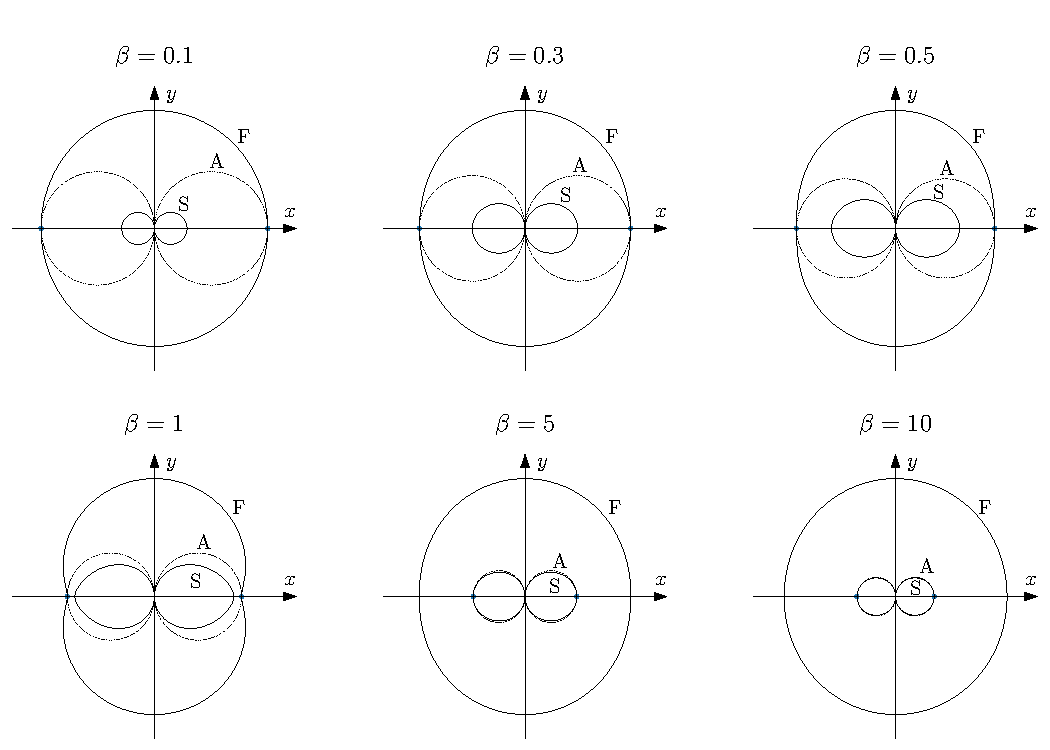
\includegraphics[width=0.8\textwidth]{../report/figures/fasespeed_beta.pdf}
		\caption{Phase speed for different $\beta$}	
	\end{figure}
\end{frame}
\begin{frame}
	\begin{figure}[h]
		\centering
		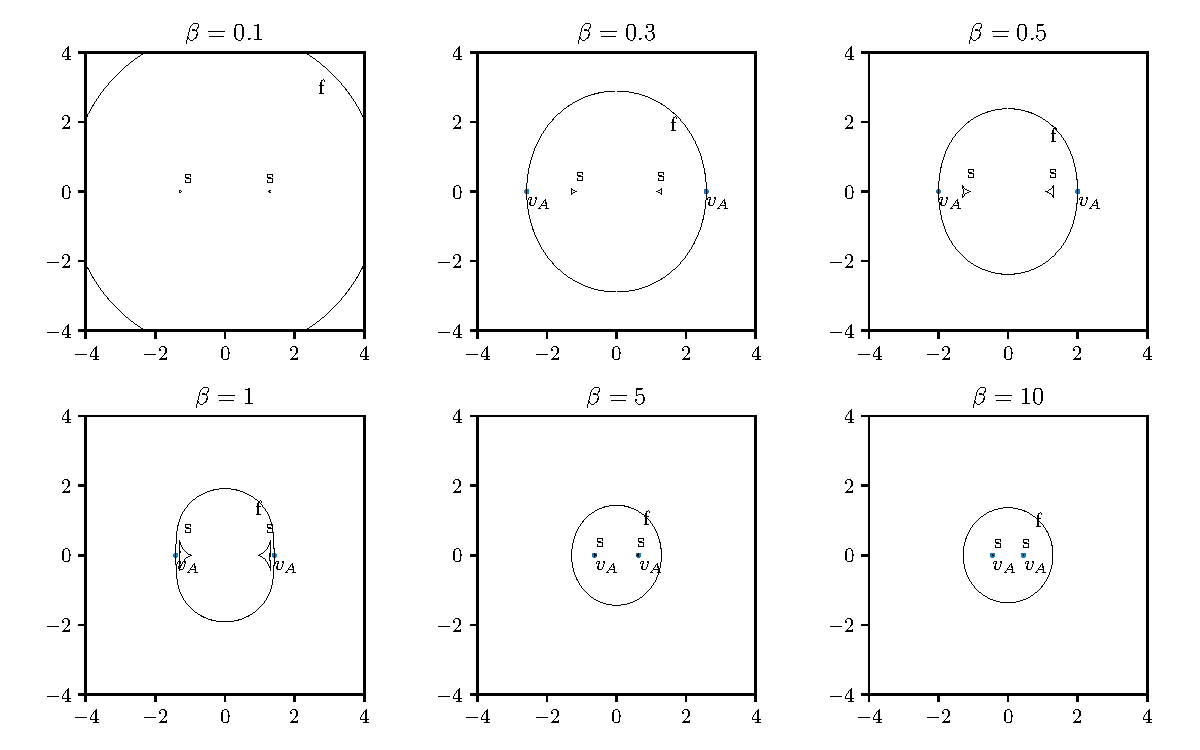
\includegraphics[width=.9\textwidth]{../report/figures/groupspeed_beta.pdf}
		\caption{Group speed for different $\beta$}
	\end{figure}	
\end{frame}

\section{PLUTO}
\begin{frame}{PLUTO}	
	The PLUTO Code for Astrophysical GasDynamics \cite{plutouserguide}
	\begin{itemize}
		\item Uncompiled
			\begin{itemize}
				\item initial/boundary conditions needs to programmed in C.
				\item binary needs to be made for specific problem
			\end{itemize} 		
		\item Solvers for many equations (HD, MHD, relativisctic MHD, \ldots)
		\item Supports many types of geometry. 
	\end{itemize}
\end{frame}
\begin{frame}{Simple blastwave}
Initial conditions:\\
\begin{minipage}{.49\linewidth}
\begin{align*}
	p &= \begin{cases}
		p_\text{in} & \text{if } r < 0.3\\
		p_\text{out} & \text{if } r > 0.3
	\end{cases} \\
	\rho &= 1 \\
	\mathbf v &=  \mathbf 0 \\
	p_\text{out}  &= 8, \quad p_\text{in}  = 15
.\end{align*}
\end{minipage}
\begin{minipage}{.49\linewidth}
	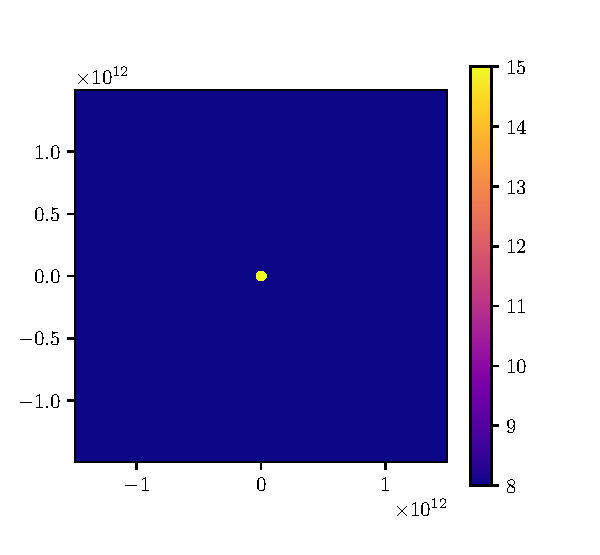
\includegraphics[width=\textwidth]{figures/initial.pdf}	
\end{minipage}
Domain: Square from $-10$ to $10$ in $ X, Y$-direction covered by $1024\times 1024$ grid.

Boundary conditions: Outflow


\end{frame}

\begin{frame}
	\begin{figure}[h]
		\centering
		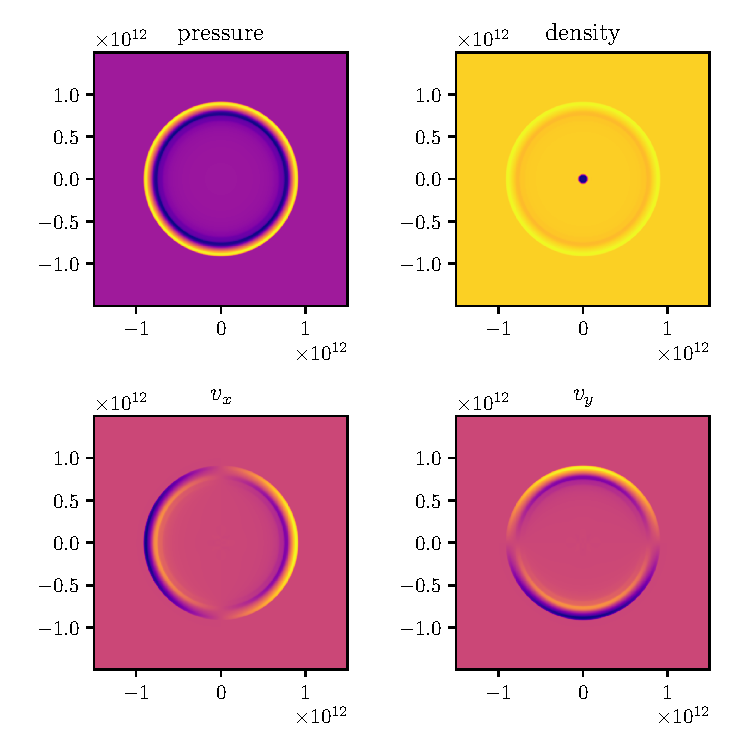
\includegraphics[width=0.75\textwidth]{figures/output.pdf}
	\end{figure}	
\end{frame}
\begin{frame}
	\begin{figure}[h]
		\centering
		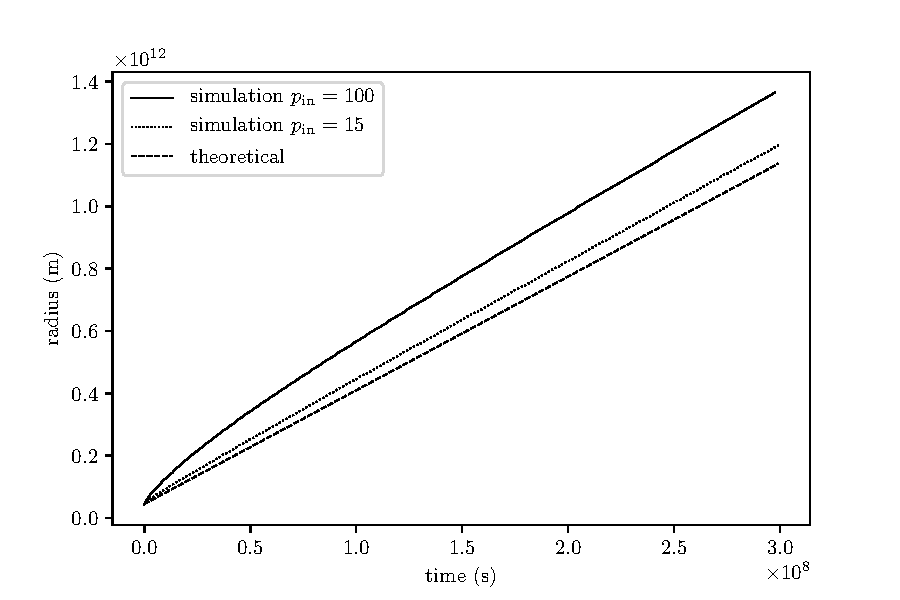
\includegraphics[width=0.8\textwidth]{figures/non_linear_effects.pdf}
	\end{figure}
\end{frame}
\section{MHD Blastwave}
\begin{frame}{MHD Blastwave}

Initial conditions:\\
\begin{minipage}{.49\linewidth}
	\begin{align*}
	p &= \begin{cases}
		p_\text{in} & \text{if } r < 0.3\\
		p_\text{out} & \text{if } r > 0.3
	\end{cases} \\
	\rho &= 1 \\
	\mathbf v &=  \mathbf 0 \\
	\mathbf B &= \sqrt{\frac{2 p_\text{out} }{\beta}} \hat{x}\\
	p_\text{out}  &= 8, \quad p_\text{in}  = 15
.\end{align*}
\end{minipage}
\begin{minipage}{.49\linewidth}
	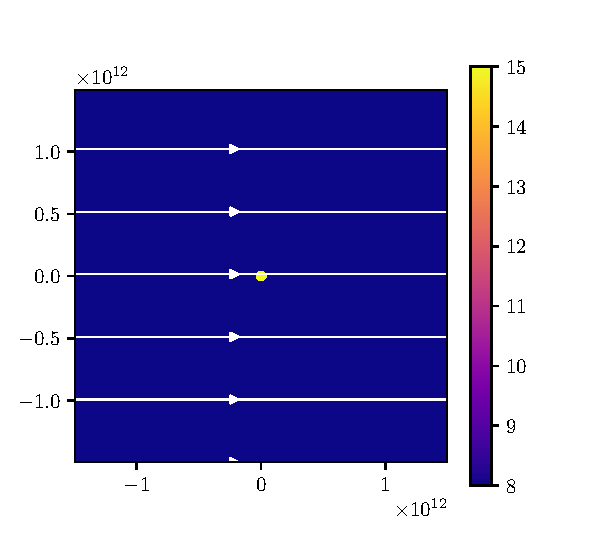
\includegraphics[width=\textwidth]{figures/initial_MHD.pdf}	
\end{minipage}
Domain: Square from $-10$ to $10$ in $ X, Y$-direction covered by $1024\times 1024$ grid.

Boundary conditions: Outflow
\end{frame}
\begin{frame}
	\begin{figure}[h]
		\centering
		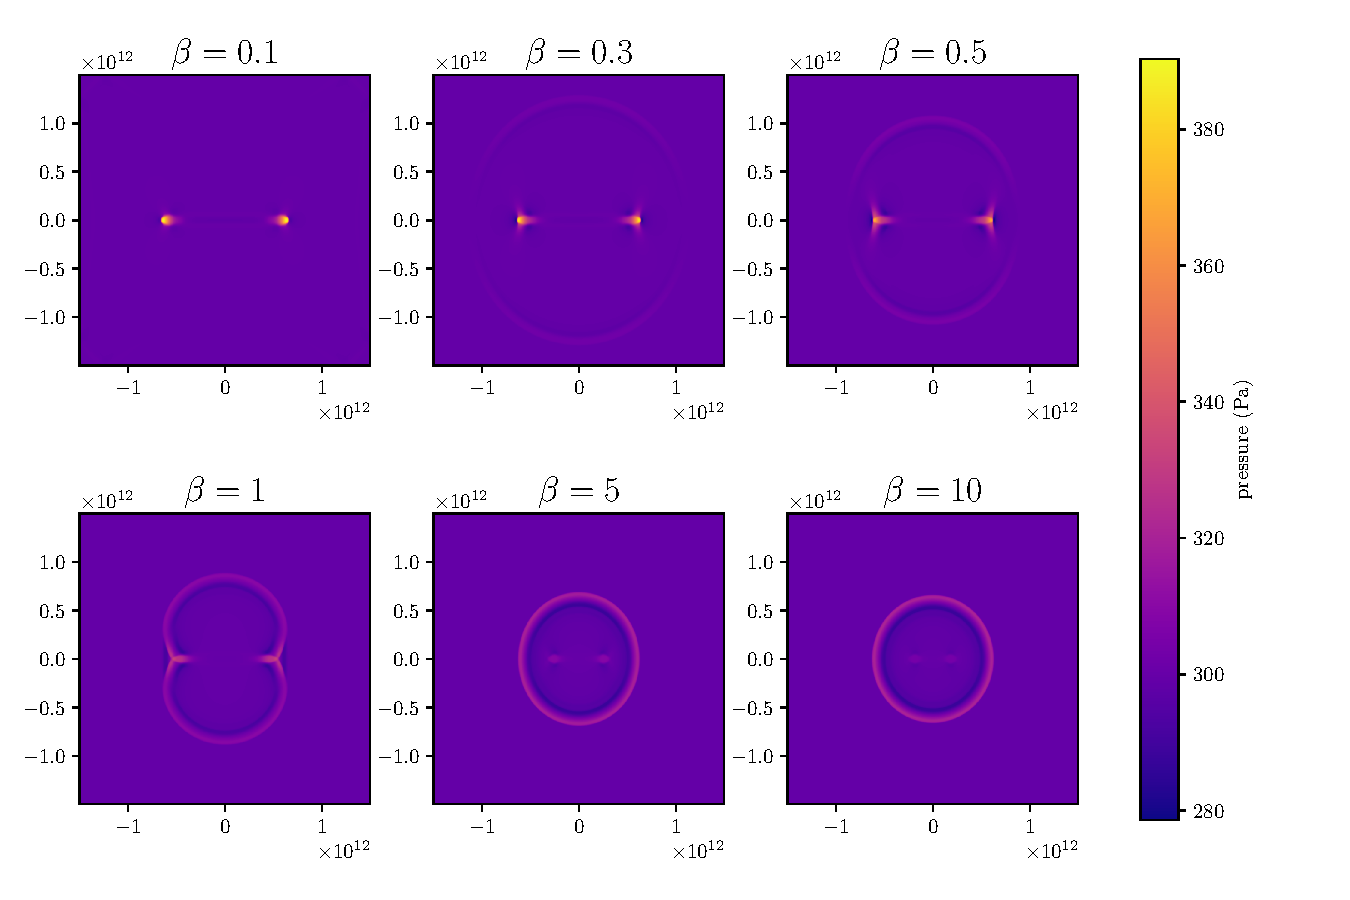
\includegraphics[width=1.1\textwidth]{figures/influence_beta.pdf}
	\end{figure}
\end{frame}
\begin{frame}
	\begin{figure}[h]
		\centering
		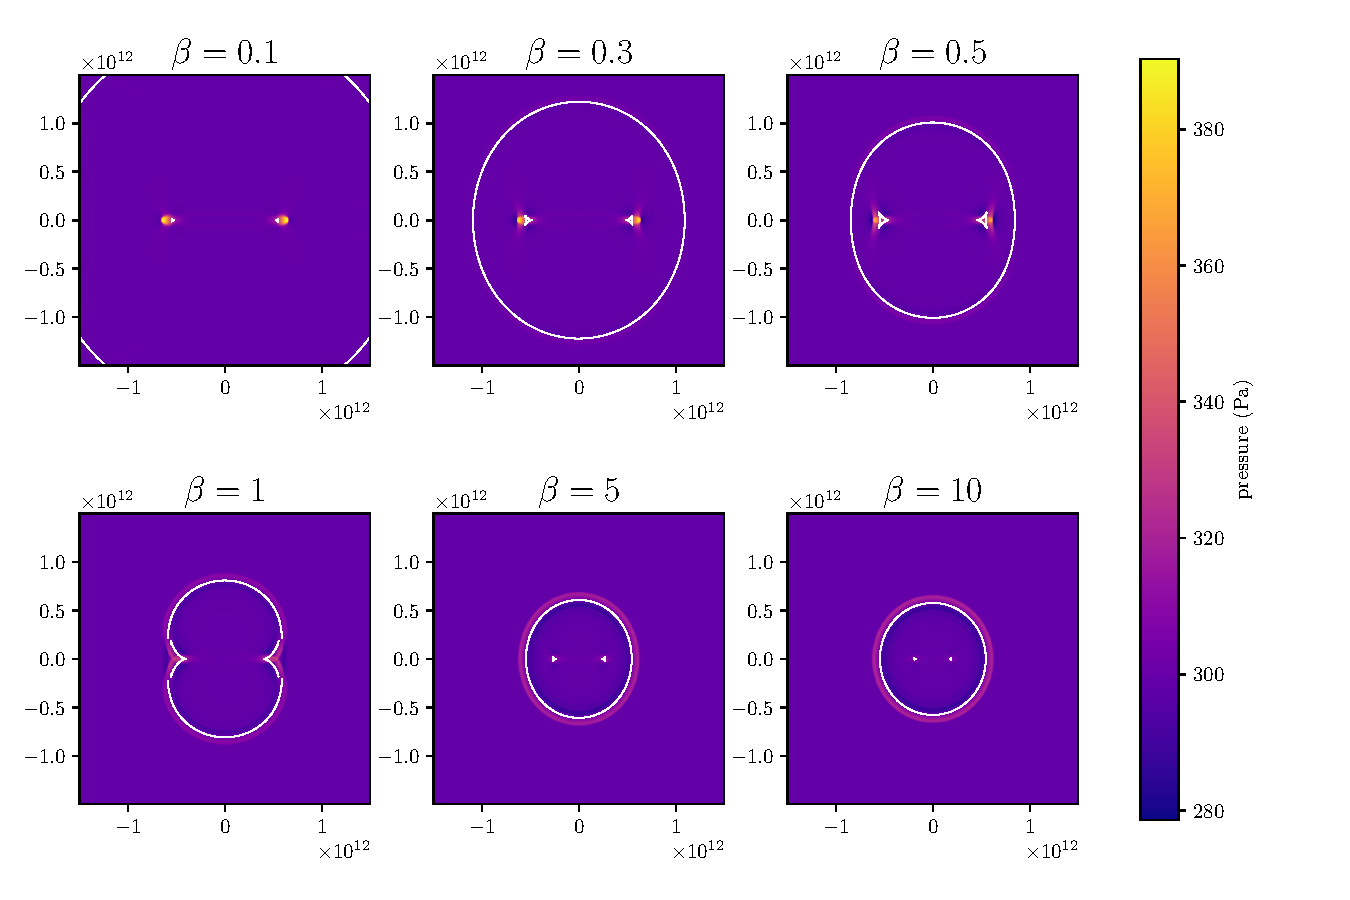
\includegraphics[width=1.1\textwidth]{figures/comparison_groupspeed.pdf}
	\end{figure}
\end{frame}
\begin{frame}
	When $\beta = 0.1$ slow waves are predominant. Ideal for analysis. 
	\begin{figure}[h]
		\centering
		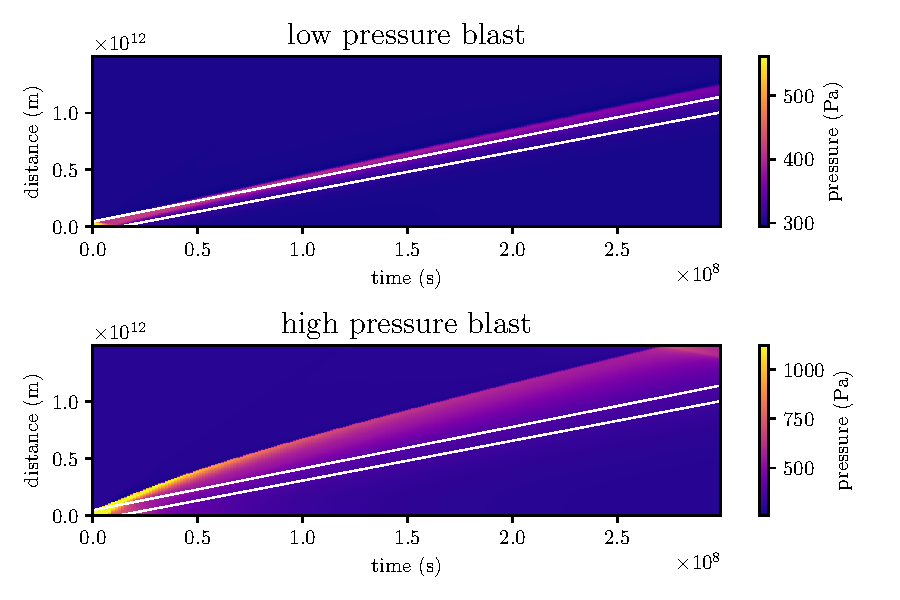
\includegraphics[width=\textwidth]{figures/slowwave_time.pdf}
	\end{figure}
\end{frame}
\section{Modelling the Solar Corona}
\begin{frame}{Coronal Holes}
	The goal is to reproduce the results of a paper by A. N. Afanasyev and A. N. Zhukov\cite{afanasyev2018propagation}.

   \bigskip 
   Coronal hole:
   \begin{itemize}
   	\item Low density/temperature region on the solar corona. 
	\item Typical size: \SI{150}{Mm}
	\item Region of high Alfv\'en speed. 
   \end{itemize}
   
\end{frame}

\begin{frame}{Model}
	Domain: square from $\SI{-1000}{\mega \metre}$ to $\SI{1000}{\mega\metre}$, covered by $1024 \times  1024$ grid. 

\medskip

	Initial conditions:
	\begin{align*}
		\rho &= \rho _\text{out} -(\rho_\text{out}  - \rho_\text{in} )\exp\left[ -\left( \frac{r}{d} \right) ^{8} \right]  \\
		T &= T_\text{out}  - (T_\text{out}  - T_\text{in} )\exp\left[ -\left( \frac{r}{d} \right)^{8}  \right] \\
		p^{t} &= p_\text{gas} + \frac{B^2}{8 \pi} = \text{constant}
	.\end{align*}
	Here $d = \SI{150}{\mega\metre},\; \rho_\text{out}  = 10^{9}m_p \si{\per \centi\metre\cubed},\; \rho_\text{in}  = 10^{8}m_p \si{\per \centi\metre\cubed},\; T_\text{out}  = \SI{1.5}{\mega\kelvin},\; T_\text{in}  = \SI{100}{\mega\kelvin}, B_\text{out}  = \SI{4}{G}$.
\end{frame}
\begin{frame}{Model}
	Boundary conditions: Top and bottom are periodic. Right is an outflow. Left drives $v_x$ using \[
		v_x = v_\text{max} \tanh\left( \frac{t}{\SI{20}{s}} \right) - \frac{v_\text{max} }{2}\left( \tanh\left( \frac{t - t_0}{\SI{60}{s}} \right) + 1 \right) 
	\] 
	to induce a wave. 
	Here $v_\text{max}  = \SI{50}{\kilo\metre\per\second}$ and $t_0 = \SI{600}{s}$.\\
	\centering
		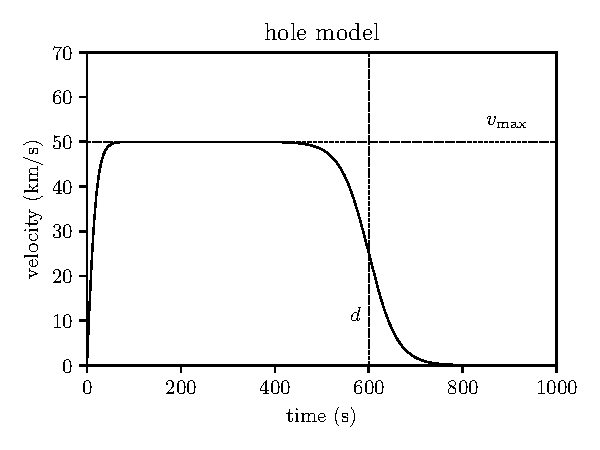
\includegraphics[width=0.5\textwidth]{figures/wave_drive.pdf}
\end{frame}
\begin{frame}
	\begin{figure}[h]
		\centering
		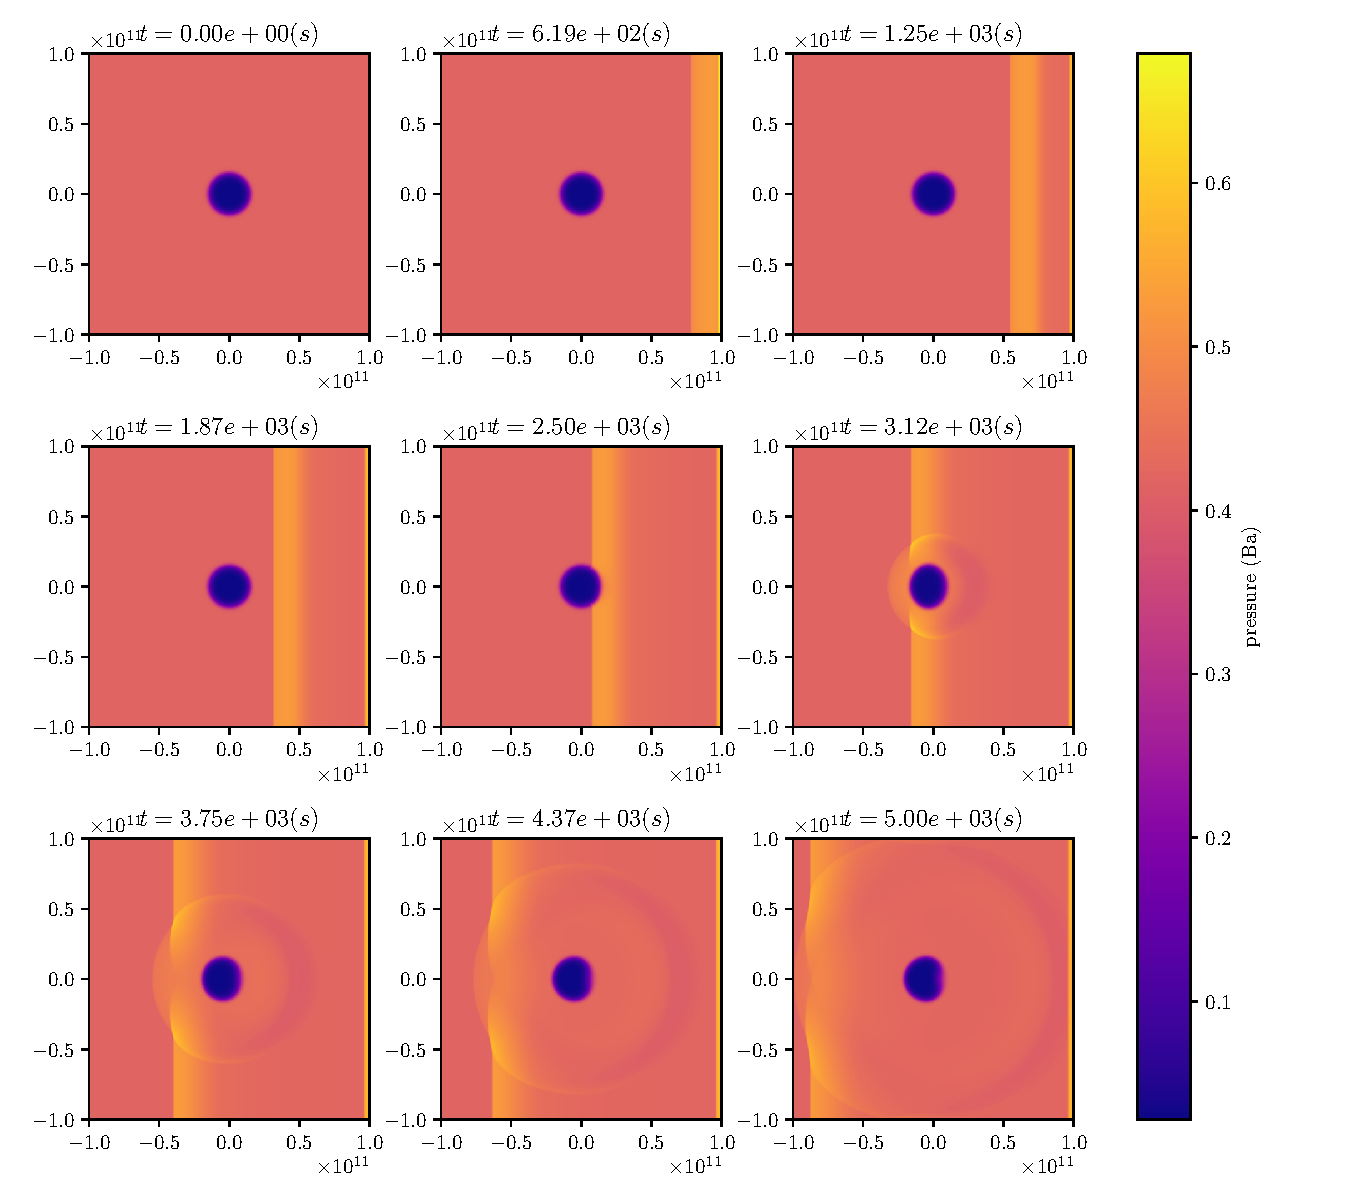
\includegraphics[width=0.88\textwidth]{../report/figures/hole_time.pdf}
	\end{figure}
\end{frame}
\begin{frame}{Analysis}
	Calculation of reflection coefficient.
	\begin{figure}[h]
		\centering
		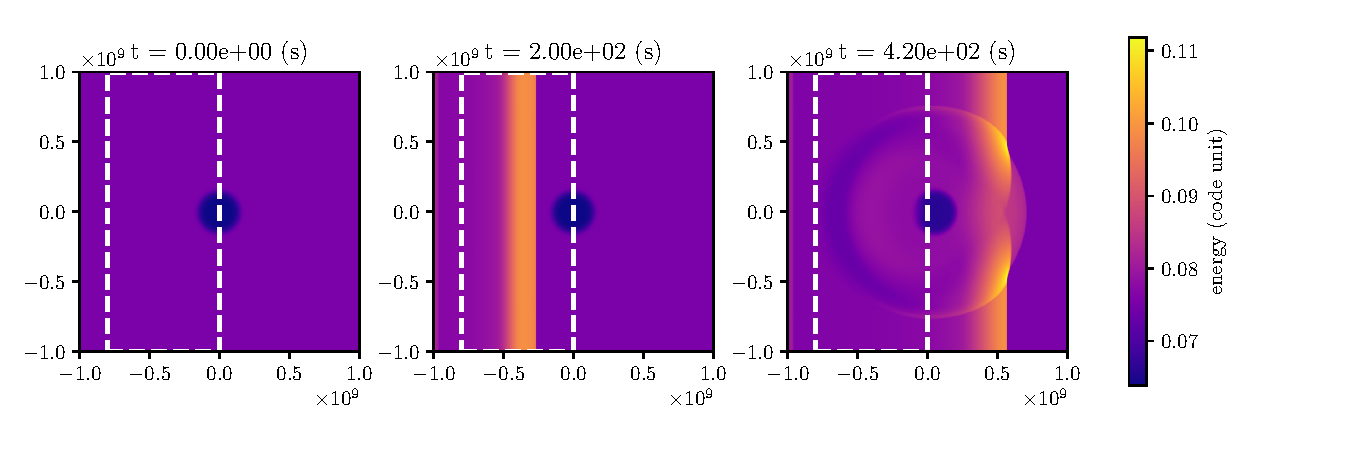
\includegraphics[width=1.1\textwidth]{figures/reflection_coefficient.pdf}
	\end{figure}	
	\[
	R = \frac{E_2 - E_0}{E_1 - E_0} = 0.17
	.\] 
\end{frame}
\section{Conclusions}
\begin{frame}
Thanks to our supervisor: Mijie Shi

\bigskip

Are there questions?
\end{frame}
\begin{frame}{References}
    \printbibliography
\end{frame}
\end{document}

